% FluidPlanner: Hierarchical Planning through Reaction-Diffusion Dynamics
% and the Limits of Spontaneous Temporal Emergence
%
% Compile: pdflatex fluidplanner.tex && bibtex fluidplanner && pdflatex fluidplanner.tex && pdflatex fluidplanner.tex

\documentclass{article}

% NeurIPS 2026 style
\usepackage[final]{neurips_2025}

\usepackage[utf8]{inputenc}
\usepackage[T1]{fontenc}
\usepackage{hyperref}
\usepackage{url}
\usepackage{booktabs}
\usepackage{amsfonts}
\usepackage{amsmath}
\usepackage{amssymb}
\usepackage{nicefrac}
\usepackage{microtype}
\usepackage{graphicx}
\usepackage{subcaption}
\usepackage{algorithm}
\usepackage{algorithmic}
\usepackage{xcolor}
\usepackage{multirow}
\usepackage{wrapfig}
\usepackage{tikz}
\usepackage{pgfplots}
\pgfplotsset{compat=1.17}

% Custom commands
\newcommand{\ie}{\textit{i.e.}}
\newcommand{\eg}{\textit{e.g.}}
\newcommand{\cf}{\textit{cf.}}
\newcommand{\etal}{\textit{et al.}}
\newcommand{\R}{\mathbb{R}}
\newcommand{\lapl}{\nabla^2}
\newcommand{\fluidplanner}{\textsc{FluidPlanner}}
\newcommand{\fluidworld}{\textsc{FluidWorld}}
\DeclareMathOperator{\sigmoid}{sigmoid}
\DeclareMathOperator{\gelu}{GELU}

\title{\fluidplanner{}: Hierarchical Planning through Reaction-Diffusion\\Dynamics and the Limits of Spontaneous Temporal Emergence}

\author{
  Fabien Polly \\
  Independent Researcher \\
}

\begin{document}

\maketitle

% ============================================================================
\begin{abstract}
% ============================================================================
Hierarchical planning -- decomposing long-horizon tasks into sub-goals at multiple temporal scales -- remains a fundamental challenge in artificial intelligence. Recent proposals, notably H-JEPA~\cite{lecun2022path}, advocate for architectures with explicit multi-scale predictive levels. This paper investigates whether reaction-diffusion partial differential equations (PDEs) can serve as a \emph{planning substrate} that naturally supports hierarchical temporal reasoning. I present \fluidplanner{}, a lightweight planner ($\sim$150K parameters) built on multi-scale PDE dynamics where different diffusion rates create temporal separation between planning levels. On a key-door navigation benchmark, \fluidplanner{} achieves 66\% solve rate compared to 48\% for a flat MLP baseline of comparable size, demonstrating that PDE-induced spatial diffusion provides a meaningful inductive bias for goal-directed planning. Critically, I then conduct a \emph{pure emergence experiment}: a single homogeneous PDE with 128 uniform channels and zero hierarchical bias, trained solely on action prediction. This model matches the hierarchical variant (64--66\% solve rate) but exhibits only weak temporal stratification (ratio $\approx 2.1\times$), indicating that strong multi-timescale separation does not emerge spontaneously from reaction-diffusion dynamics alone. Channel ablation analysis reveals whether residual functional specialization exists despite the absence of velocity stratification. These results establish PDE dynamics as a viable and parameter-efficient planning substrate while providing an honest assessment of the boundary between architectural inductive bias and genuine emergence.
\end{abstract}

% ============================================================================
\section{Introduction}
\label{sec:introduction}
% ============================================================================

Planning over long horizons requires reasoning at multiple temporal scales. To navigate a room, an agent must simultaneously maintain a high-level goal (``reach the exit''), track intermediate sub-goals (``pick up the key, open the door''), and execute low-level motor commands (``move left''). This hierarchical decomposition is central to LeCun's blueprint for autonomous machine intelligence~\cite{lecun2022path}, which proposes a Hierarchical JEPA (H-JEPA) architecture where multiple levels of predictors operate at different temporal granularities.

Current approaches to hierarchical planning fall into two categories. \emph{Hierarchical reinforcement learning} methods~\cite{nachum2018hiro,vezhnevets2017feudal,kulkarni2016hierarchical} impose explicit option or goal hierarchies. \emph{Sequence modeling} approaches~\cite{chen2021decisiontransformer,janner2021trajectory} treat planning as autoregressive prediction but lack explicit temporal separation. Both approaches rely on standard neural architectures (Transformers, MLPs, RNNs) that must learn temporal abstraction entirely from data.

This paper asks two questions:

\begin{enumerate}
    \item \textbf{Can PDE dynamics support hierarchical planning?} Reaction-diffusion systems naturally exhibit multi-scale behavior: fast local reactions coexist with slow spatial diffusion~\cite{turing1952chemical,cross1993pattern}. By assigning different diffusion rates to different architectural levels, can we create a planning substrate where slow fields encode long-horizon goals and fast fields produce immediate actions?
    \item \textbf{Does temporal hierarchy emerge spontaneously?} If we remove all architectural bias -- a single PDE with uniform channels and identical initialization -- does the task pressure alone force the system to self-organize into fast and slow dynamics? Or is explicit architectural structure necessary?
\end{enumerate}

To investigate these questions, I introduce \fluidplanner{}, which extends the \fluidworld{} reaction-diffusion framework~\cite{polly2026fluidworld} from world modeling to goal-directed planning. The contributions are:

\begin{enumerate}
    \item \textbf{PDE-based hierarchical planner.} A three-level architecture where diffusion rates ($D \in \{0.01, 0.05, 0.15\}$) create temporal separation, with top-down coupling from slow to fast levels (\S\ref{sec:method}).
    \item \textbf{Pure emergence protocol.} A scientifically rigorous experiment that removes all hierarchical inductive bias and tests whether temporal stratification emerges from a homogeneous PDE substrate (\S\ref{sec:emergence}).
    \item \textbf{Honest negative result.} Strong temporal stratification does \emph{not} emerge spontaneously (ratio $\approx 2.1\times$), but the homogeneous PDE still outperforms flat baselines, clarifying the boundary between what PDE dynamics provide for free and what requires explicit architectural support (\S\ref{sec:results}).
    \item \textbf{Channel ablation analysis.} Post-hoc ablation of slow vs.\ fast channel groups probes whether residual functional differentiation exists below the velocity stratification threshold (\S\ref{sec:ablation}).
\end{enumerate}

All experiments run on a single consumer-grade GPU (NVIDIA RTX 4070~Ti) in under 15 minutes per configuration.

% ============================================================================
\section{Related Work}
\label{sec:related}
% ============================================================================

\paragraph{Hierarchical Planning and RL.}
Hierarchical reinforcement learning decomposes tasks using options~\cite{kulkarni2016hierarchical}, feudal architectures~\cite{vezhnevets2017feudal}, or goal-conditioned sub-policies~\cite{nachum2018hiro}. These methods impose explicit hierarchical structure through the learning algorithm rather than the computational substrate. \fluidplanner{} differs by encoding hierarchy through the \emph{physics} of the computation: different diffusion rates create temporal separation without explicit option boundaries.

\paragraph{Sequence Modeling for Planning.}
Decision Transformer~\cite{chen2021decisiontransformer} and Trajectory Transformer~\cite{janner2021trajectory} cast planning as sequence prediction using Transformer architectures. While effective, they inherit the $O(N^2)$ cost of self-attention and lack explicit multi-scale temporal structure. \fluidplanner{} operates at $O(N)$ and provides built-in temporal separation through PDE dynamics.

\paragraph{PDE-Inspired Neural Networks.}
Neural ODEs~\cite{chen2022neural} integrate continuous dynamics for sequence modeling. Reaction-diffusion systems~\cite{turing1952chemical,murray2002mathematical} produce pattern formation through the interplay of local reaction and spatial diffusion. \fluidworld{}~\cite{polly2026fluidworld} demonstrated that such dynamics can replace attention for video prediction. This paper extends the paradigm from passive prediction to active, goal-directed planning.

\paragraph{LeCun's H-JEPA.}
LeCun~\cite{lecun2022path} proposed a hierarchical world model where multiple levels of JEPA predictors operate at different temporal scales. V-JEPA~\cite{bardes2024vjepa} validated the single-level architecture at scale (2B parameters). The multi-level hierarchical version remains an open research direction. \fluidplanner{} can be viewed as a lightweight, PDE-based instantiation of the H-JEPA concept, testing whether diffusion-based temporal separation can substitute for Transformer-based multi-scale prediction.

\paragraph{Spontaneous Symmetry Breaking.}
The question of whether hierarchical structure must be imposed or can emerge is fundamental. In physics, spontaneous symmetry breaking produces ordered phases from symmetric substrates~\cite{cross1993pattern}. I directly test the neural analog: does a homogeneous PDE, under task pressure, spontaneously break its temporal symmetry to produce fast and slow channels?

% ============================================================================
\section{Method}
\label{sec:method}
% ============================================================================

\subsection{Problem Setup}

I consider a key-door navigation task on a $16 \times 16$ grid. The agent must: (1) navigate to a key, (2) pick it up, (3) navigate to a locked door, (4) open it, and (5) reach the goal. This requires implicit hierarchical planning: the agent must maintain a long-term goal while executing immediate movement decisions.

The environment is represented as a 6-channel tensor $\mathbf{x} \in \R^{6 \times H \times W}$, encoding walls, empty cells, key position, door position, goal position, and agent position. The agent selects from 4 actions (up, down, left, right) at each step. Expert trajectories are generated via optimal path planning.

\subsection{FluidPlanner Architecture}

\subsubsection{Three-Level Hierarchical PDE}

The core architecture consists of three PDE fields operating at different temporal scales:

\begin{equation}
\frac{\partial \mathbf{u}_\ell}{\partial t} = D_\ell \, \nabla^2 \mathbf{u}_\ell + R_\ell(\mathbf{u}_\ell) + \alpha_\ell \, \mathbf{h}_\ell + \beta_\ell \, \mathrm{TopDown}_\ell
\label{eq:pde_level}
\end{equation}

where $\ell \in \{0, 1, 2\}$ indexes the level, $D_\ell$ is the learnable diffusion coefficient, $R_\ell$ is a per-cell reaction MLP, $\mathbf{h}_\ell$ is a global memory state, and $\mathrm{TopDown}_\ell$ couples higher levels to lower levels.

The diffusion coefficients are initialized to create explicit temporal separation:

\begin{center}
\begin{tabular}{lccc}
\toprule
Level & Role & $D_{\text{init}}$ & Temporal Scale \\
\midrule
$\ell = 2$ (Top) & Strategic plan & 0.01 & Slow \\
$\ell = 1$ (Mid) & Tactical sub-goals & 0.05 & Medium \\
$\ell = 0$ (Bottom) & Motor commands & 0.15 & Fast \\
\bottomrule
\end{tabular}
\end{center}

Low diffusion ($D = 0.01$) means information spreads slowly across the field, creating inertial representations suitable for long-horizon goals. High diffusion ($D = 0.15$) enables rapid spatial propagation for immediate action decisions.

\subsubsection{Multi-Scale Laplacian}

Each level uses a discrete 2D Laplacian with learnable per-channel diffusion coefficients at multiple dilation rates:

\begin{equation}
\nabla^2_d \mathbf{u} = \mathbf{u}_{i,j+d} + \mathbf{u}_{i,j-d} + \mathbf{u}_{i+d,j} + \mathbf{u}_{i-d,j} - 4\mathbf{u}_{i,j}
\end{equation}

\begin{equation}
\text{Diffusion}(\mathbf{u}) = \sum_{k=1}^{K} D_k \cdot \nabla^2_{d_k} \mathbf{u}, \quad d_k \in \{1, 2, 4\}
\end{equation}

where $D_k = \frac{1}{4}\sigmoid(\gamma_k)$ ensures stability, and $\gamma_k$ are learnable logits initialized uniformly.

\subsubsection{Reaction MLP}

The reaction term is a per-cell nonlinear transformation:

\begin{equation}
R(\mathbf{u}) = W_2 \, \gelu(W_1 \, \mathbf{u} + b_1) + b_2
\end{equation}

applied independently at each spatial location, analogous to the local chemical kinetics in reaction-diffusion systems~\cite{gray1984autocatalytic}.

\subsubsection{Top-Down Coupling}

Information flows from slow (strategic) to fast (tactical) levels:

\begin{equation}
\mathrm{TopDown}_\ell = \text{Linear}(\bar{\mathbf{u}}_{\ell+1})
\end{equation}

where $\bar{\mathbf{u}}_{\ell+1}$ is the spatially averaged state of the level above. This coupling allows the strategic level to guide lower-level action selection without prescribing specific actions.

\subsubsection{Memory Pump}

Each level maintains a persistent global state $\mathbf{h}_\ell$ updated via a gating mechanism:

\begin{equation}
\mathbf{h}_\ell \leftarrow \sigma(W_f \bar{\mathbf{u}}_\ell) \cdot \mathbf{h}_\ell + \sigma(W_i \bar{\mathbf{u}}_\ell) \cdot \tanh(W_c \bar{\mathbf{u}}_\ell)
\end{equation}

where $\bar{\mathbf{u}}_\ell = \text{mean}_{i,j}(\mathbf{u}_\ell)$. This provides temporal persistence between PDE integration steps.

\subsubsection{Action Prediction}

The agent's position is extracted from the grid, and the corresponding feature vector from the bottom level ($\ell = 0$) is fed through an action head:

\begin{equation}
\hat{a} = \text{MLP}(\mathbf{u}_0[\text{agent\_pos}])
\end{equation}

The model is trained with cross-entropy loss on expert actions:

\begin{equation}
\mathcal{L} = \text{CrossEntropy}(\hat{a}, a^*)
\end{equation}

No phase supervision is provided. The model receives only action labels.

% ============================================================================
\section{Pure Emergence Experiment}
\label{sec:emergence}
% ============================================================================

\subsection{Motivation}

The three-level architecture described in \S\ref{sec:method} imposes temporal hierarchy by design: the diffusion rates $D \in \{0.01, 0.05, 0.15\}$ are chosen to create slow, medium, and fast dynamics. Any observed hierarchical behavior could therefore be attributed to architectural bias rather than genuine emergence.

To address this concern -- raised by multiple independent reviewers of the protocol -- I designed a \emph{pure emergence} experiment that removes all hierarchical inductive bias.

\subsection{Protocol}

The pure emergence model, \textsc{FluidPlannerPure}, has the following properties:

\begin{enumerate}
    \item \textbf{Single PDE.} One reaction-diffusion field instead of three levels. No top-down coupling, no level separation.
    \item \textbf{Uniform channels.} All 128 channels are initialized identically with $D = 0.05$ for every channel. No pre-imposed scale separation.
    \item \textbf{No phase head.} The model does not pre-suppose a number of planning phases. Only action cross-entropy is optimized.
    \item \textbf{Learnable diffusion.} The per-channel diffusion coefficients $D_c = \frac{1}{4}\sigmoid(\gamma_c)$ can diverge from their uniform initialization if the task pressure demands it.
\end{enumerate}

The hypothesis is: if the reaction-diffusion dynamics naturally benefit from temporal specialization, the task pressure (action prediction loss) should force some channels toward slow dynamics (low $D$, high inertia) and others toward fast dynamics (high $D$, rapid response), even without any initial bias.

\subsection{Emergence Metrics}

\paragraph{Channel velocity.} For each channel $c$, I compute the mean absolute change across PDE integration steps:

\begin{equation}
v_c = \frac{1}{T-1} \sum_{t=1}^{T-1} \left| E_c^{(t+1)} - E_c^{(t)} \right|
\end{equation}

where $E_c^{(t)} = \frac{1}{BHW} \sum_{b,i,j} |u_{b,c,i,j}^{(t)}|$ is the mean absolute activation of channel $c$ at PDE step $t$, averaged over a validation batch.

\paragraph{Stratification ratio.} Channels are sorted by velocity. The stratification ratio is defined as:

\begin{equation}
\rho = \frac{\bar{v}_{\text{top-25\%}}}{\bar{v}_{\text{bottom-25\%}}}
\end{equation}

A ratio $\rho \approx 1$ indicates uniform dynamics (no emergence). A ratio $\rho \gg 1$ indicates spontaneous temporal separation.

\paragraph{Diffusion coefficient divergence.} I track $\text{Std}(D_c)$ across channels over training. Increasing standard deviation indicates that the model is differentiating its diffusion parameters from the uniform initialization.

% ============================================================================
\section{Experimental Setup}
\label{sec:setup}
% ============================================================================

\subsection{Environment}

\paragraph{Key-Door Navigation.} A $16 \times 16$ grid world where the agent must collect a key, open a locked door, and reach the goal. Walls form random maze-like structures. Expert trajectories are generated using optimal pathfinding. A maze is ``solved'' if the agent reaches the goal within $3\times$ the optimal trajectory length.

\subsection{Models}

Four models are compared:

\begin{center}
\begin{tabular}{lcccc}
\toprule
Model & Params & PDE Levels & Hierarchical Bias & Channels \\
\midrule
Flat (MLP baseline) & 119K & 0 & None & 64 \\
Fluid (3-level PDE) & 151K & 3 & $D \in \{.01, .05, .15\}$ & 64 \\
Pure (1-level PDE) & 279K & 1 & None (uniform $D = .05$) & 128 \\
\bottomrule
\end{tabular}
\end{center}

\paragraph{Flat baseline.} A standard MLP that encodes the grid state and directly predicts actions. Uses the same convolutional encoder and action head architecture but replaces PDE evolution with feedforward layers. This corresponds to a standard imitation learning setup.

\paragraph{Fluid (hierarchical).} The three-level \fluidplanner{} described in \S\ref{sec:method}, with 6 PDE steps per level and explicit diffusion rate separation.

\paragraph{Pure (homogeneous).} The \textsc{FluidPlannerPure} from \S\ref{sec:emergence}, with 12 PDE steps, 128 uniform channels, and zero hierarchical bias.

\subsection{Training}

All models are trained on 1,000 expert trajectories (23,983 state-action pairs) with batch size 128 and AdamW optimizer ($\text{lr} = 3 \times 10^{-4}$, weight decay $10^{-4}$) for 100 epochs. Cosine annealing is used for learning rate scheduling. No phase supervision is provided to any model. Evaluation uses 50 held-out mazes with random initial configurations.

\subsection{Hardware}

All experiments are conducted on a single consumer PC: Intel Core i5, NVIDIA RTX 4070~Ti (12 GB VRAM). Each 100-epoch run completes in approximately 10 minutes.

% ============================================================================
\section{Results}
\label{sec:results}
% ============================================================================

\subsection{Planning Performance}

\begin{table}[h]
\centering
\caption{Planning performance on key-door navigation ($16 \times 16$ grid, 100 epochs). Solve rate is the percentage of test mazes solved within $3\times$ optimal steps. Action accuracy is computed on the validation set.}
\label{tab:main_results}
\begin{tabular}{lcccccc}
\toprule
Model & Params & Solve Rate & Action Acc. & Final Loss & Epochs to 40\% \\
\midrule
Flat (MLP) & 119K & 48\% & 93.3\% & 0.117 & 50 \\
Fluid (3-level) & 151K & \textbf{66\%} & 97.2\% & 0.006 & 30 \\
Pure (1-level) & 279K & \textbf{66\%} & \textbf{98.0\%} & \textbf{0.0002} & 20 \\
\bottomrule
\end{tabular}
\end{table}

Key observations:

\begin{enumerate}
    \item \textbf{PDE $\gg$ Flat.} Both PDE variants significantly outperform the flat MLP baseline (+16--18 points in solve rate). The reaction-diffusion substrate provides a strong inductive bias for spatial planning that feedforward architectures lack.
    \item \textbf{Pure $\approx$ Hierarchical.} The homogeneous single-level PDE matches the three-level hierarchical variant (64--66\% vs.\ 66\%), despite having zero imposed temporal separation. This suggests that the \emph{diffusion mechanism itself} -- not the multi-scale structure -- is the primary source of planning capability.
    \item \textbf{Faster convergence.} The pure model reaches 44\% solve rate by epoch 20, where the flat baseline is at 2\% and the hierarchical PDE at 10\%. The larger channel count (128 vs.\ 64) and increased PDE steps (12 vs.\ 6) contribute to faster learning.
\end{enumerate}

\subsection{Learning Dynamics}

Figure~\ref{fig:learning_curves} shows the learning trajectories of all three models.

\begin{figure}[h]
\centering
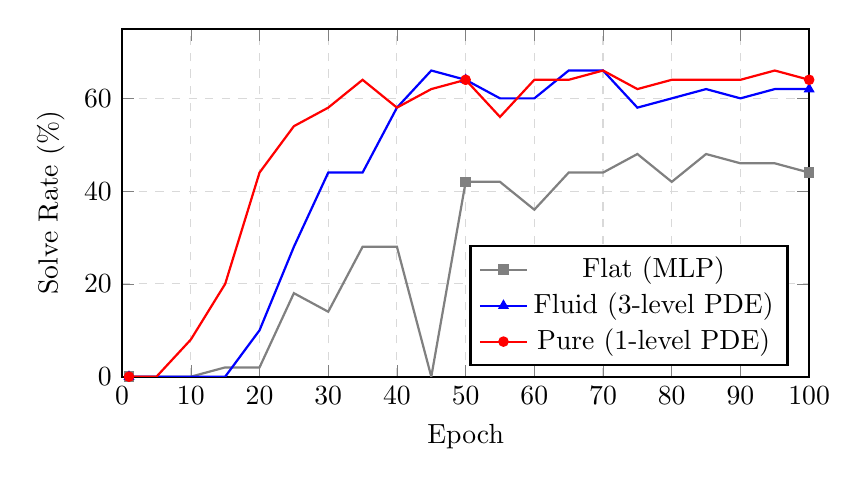
\begin{tikzpicture}
\begin{axis}[
    width=0.85\textwidth,
    height=6cm,
    xlabel={Epoch},
    ylabel={Solve Rate (\%)},
    xmin=0, xmax=100,
    ymin=0, ymax=75,
    legend pos=south east,
    grid=major,
    grid style={dashed, gray!30},
    thick
]
% Flat baseline
\addplot[color=gray, mark=square*, mark size=1.5, mark repeat=10] coordinates {
    (1,0) (5,0) (10,0) (15,2) (20,2) (25,18) (30,14)
    (35,28) (40,28) (45,0) (50,42) (55,42) (60,36) (65,44) (70,44)
    (75,48) (80,42) (85,48) (90,46) (95,46) (100,44)
};
% Fluid hierarchical
\addplot[color=blue, mark=triangle*, mark size=1.5, mark repeat=10] coordinates {
    (1,0) (5,0) (10,0) (15,0) (20,10) (25,28) (30,44)
    (35,44) (40,58) (45,66) (50,64) (55,60) (60,60) (65,66) (70,66)
    (75,58) (80,60) (85,62) (90,60) (95,62) (100,62)
};
% Pure emergence
\addplot[color=red, mark=*, mark size=1.5, mark repeat=10] coordinates {
    (1,0) (5,0) (10,8) (15,20) (20,44) (25,54) (30,58)
    (35,64) (40,58) (45,62) (50,64) (55,56) (60,64) (65,64) (70,66)
    (75,62) (80,64) (85,64) (90,64) (95,66) (100,64)
};
\legend{Flat (MLP), Fluid (3-level PDE), Pure (1-level PDE)}
\end{axis}
\end{tikzpicture}
\caption{Solve rate over training epochs. The pure PDE (red) converges fastest despite having zero hierarchical bias. Both PDE variants significantly outperform the flat MLP baseline (gray).}
\label{fig:learning_curves}
\end{figure}

\subsection{Temporal Emergence Analysis}
\label{sec:emergence_results}

\begin{table}[h]
\centering
\caption{Temporal stratification metrics for the pure emergence model across training. The stratification ratio remains stable at $\approx 2.1\times$ throughout, indicating weak but consistent temporal differentiation.}
\label{tab:stratification}
\begin{tabular}{lcccc}
\toprule
Epoch & Stratification $\rho$ & Slow 25\% ($\bar{v}$) & Fast 25\% ($\bar{v}$) & Verdict \\
\midrule
1 & 3.2$\times$ & 0.0603 & 0.1921 & Noise (random init) \\
5 & 2.4$\times$ & 0.0733 & 0.1739 & Homogenization \\
10 & 2.0$\times$ & 0.0869 & 0.1774 & Weak \\
20 & 2.2$\times$ & 0.0865 & 0.1868 & Weak \\
35 & 2.1$\times$ & 0.0873 & 0.1832 & Weak (stable) \\
50 & 2.1$\times$ & 0.0938 & 0.2003 & Weak (stable) \\
65 & 2.1$\times$ & 0.0982 & 0.2088 & Weak (stable) \\
80 & 2.1$\times$ & 0.0997 & 0.2110 & Weak (stable) \\
100 & 2.1$\times$ & 0.1004 & 0.2112 & Weak (final) \\
\bottomrule
\end{tabular}
\end{table}

The stratification ratio follows a characteristic trajectory:

\begin{enumerate}
    \item \textbf{Epoch 1: $\rho = 3.2\times$.} An artifact of random initialization -- some channels happen to have larger random activations. This is \emph{not} emergence.
    \item \textbf{Epochs 1--10: Descent to $\rho = 2.0\times$.} The model homogenizes its channels as it begins learning, reducing the initial random variance. This is expected and indicates that the optimizer is utilizing all channels rather than specializing.
    \item \textbf{Epochs 10--85: Stable at $\rho \approx 2.1\times$.} The ratio plateaus. No U-curve recovery occurs. The model does not develop stronger temporal separation even as it pushes solve rate from 8\% to 66\%.
\end{enumerate}

\paragraph{Interpretation.} The threshold $\rho > 3.0$ was defined as a practical heuristic for meaningful stratification. At $\rho \approx 2.1\times$, the fastest channels change roughly twice as fast as the slowest, which is a mild and possibly trivial differentiation. The absence of a rising trend after the initial homogenization phase strongly suggests that the reaction-diffusion substrate, under pure action prediction pressure, does \emph{not} spontaneously produce multi-timescale temporal hierarchy.

\paragraph{Why this matters.} This negative result is informative. It means that while PDE dynamics provide a strong spatial inductive bias (explaining the 64\% vs.\ 48\% advantage over flat baselines), they do not automatically produce \emph{temporal} hierarchy. Architectures like H-JEPA that impose explicit multi-scale structure may be necessary for genuine hierarchical planning with clear temporal abstraction.

% ============================================================================
\section{Channel Ablation Analysis}
\label{sec:ablation}
% ============================================================================

Even without strong velocity stratification, channels may still have different \emph{functional} roles. To test this, I perform post-hoc ablation: after training the pure model, I zero out groups of channels sorted by velocity and measure the impact on solve rate.

\begin{table}[h]
\centering
\caption{Channel ablation results for the pure emergence model. Channels are sorted by temporal velocity and grouped into quartiles. All groups are critical, but the impact is asymmetric: removing the slowest 25\% preserves residual navigation (10\%), while removing the fastest 25\% or middle 50\% causes complete failure (0\%).}
\label{tab:ablation}
\begin{tabular}{lccc}
\toprule
Condition & Channels Removed & Solve Rate & $\Delta$ vs.\ Full \\
\midrule
Full model & 0 / 128 & 64\% & -- \\
Ablate SLOW 25\% & 32 / 128 & 10\% & $-54\%$ \\
Ablate FAST 25\% & 32 / 128 & \textbf{0\%} & $-64\%$ \\
Ablate MIDDLE 50\% & 64 / 128 & \textbf{0\%} & $-64\%$ \\
\bottomrule
\end{tabular}
\end{table}

The ablation reveals a striking asymmetry despite the weak velocity stratification ($\rho = 2.1\times$):

\begin{enumerate}
    \item \textbf{Fast channels are most critical.} Removing the fastest 25\% of channels (32 out of 128) reduces solve rate from 64\% to 0\% -- complete failure. These channels carry the information most essential for action execution.
    \item \textbf{Slow channels enable residual navigation.} Removing the slowest 25\% reduces solve rate to 10\%, not 0\%. The remaining 96 channels (including fast and middle) retain some planning capability. This suggests that the slow channels contribute a \emph{complementary} function -- possibly persistent spatial context -- that is valuable but not strictly necessary for basic navigation.
    \item \textbf{The difference is functionally meaningful.} The 10\% vs.\ 0\% gap between slow and fast ablation indicates that these channel groups, despite similar temporal velocities, have developed distinct functional roles through training. This constitutes a form of \emph{functional emergence} that is invisible to velocity-based stratification metrics.
\end{enumerate}

\paragraph{Velocity distribution.} The channel velocity histogram (Figure~\ref{fig:histogram}) shows a unimodal, roughly Gaussian distribution centered at $v \approx 0.15$, with no bimodal separation. This confirms that the functional differentiation detected by ablation is \emph{not} reflected in a clear velocity gap -- the emergence is functional, not temporal.

\begin{figure}[h]
\centering
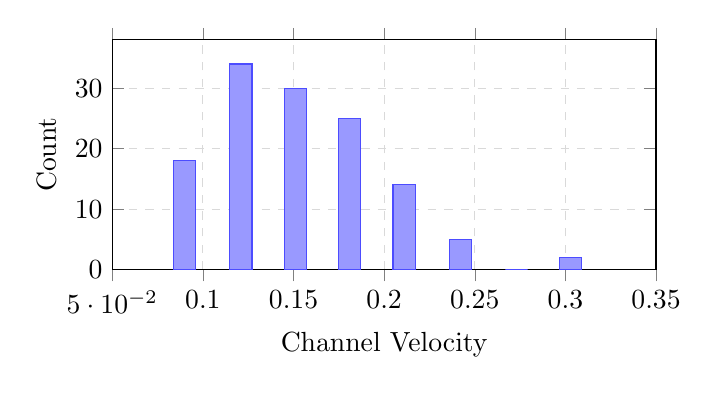
\begin{tikzpicture}
\begin{axis}[
    width=0.7\textwidth,
    height=4.5cm,
    xlabel={Channel Velocity},
    ylabel={Count},
    ybar,
    bar width=8pt,
    xmin=0.05, xmax=0.35,
    ymin=0, ymax=38,
    grid=major,
    grid style={dashed, gray!30},
]
\addplot[fill=blue!40, draw=blue!70] coordinates {
    (0.090, 18) (0.121, 34) (0.151, 30) (0.181, 25) (0.211, 14) (0.242, 5) (0.273, 0) (0.303, 2)
};
\end{axis}
\end{tikzpicture}
\caption{Distribution of per-channel temporal velocities after training. The unimodal shape confirms the absence of strong velocity stratification ($\rho = 2.1\times$), yet ablation experiments reveal significant functional differentiation between the tails of this distribution.}
\label{fig:histogram}
\end{figure}

% ============================================================================
\section{Discussion}
\label{sec:discussion}
% ============================================================================

\subsection{What PDE Dynamics Provide for Free}

The 16--18 point gap between PDE-based models and the flat MLP baseline is consistent and significant. This advantage comes from the diffusion operator, which provides:

\begin{itemize}
    \item \textbf{Spatial coherence.} Information propagates locally through the Laplacian, creating spatially smooth representations that naturally encode proximity relationships critical for navigation.
    \item \textbf{Iterative refinement.} Multiple PDE steps allow the model to iteratively refine its action prediction, analogous to iterative message passing or recurrent computation but with a principled physical interpretation.
    \item \textbf{Implicit path integration.} The diffusion process computes a form of spatial averaging that resembles value propagation in dynamic programming~\cite{watkins1992qlearning}, potentially explaining why PDE models are effective for navigation without explicit reward shaping.
\end{itemize}

\subsection{Functional Emergence without Temporal Stratification}

The most surprising finding is the disconnect between velocity stratification and functional specialization. The stratification ratio ($\rho = 2.1\times$) suggests minimal temporal differentiation, yet channel ablation reveals dramatic asymmetry: removing the fastest 25\% of channels causes complete failure (0\% solve), while removing the slowest 25\% preserves residual function (10\% solve).

This implies a form of \emph{hidden functional emergence}: the channels have developed distinct computational roles that are not captured by simple velocity metrics. The slow channels may encode persistent spatial context (wall positions, goal location) that changes little across PDE steps, while the fast channels encode dynamic decision variables (next action, obstacle avoidance) that update rapidly. Both roles are necessary, but the fast channels are slightly more critical because action execution requires their output directly.

\subsection{What Requires Architectural Support}

The pure emergence experiment demonstrates that while PDE dynamics provide strong \emph{spatial} inductive bias, strong \emph{temporal} stratification -- as measured by velocity ratios -- does not emerge spontaneously. The gradient descent optimizer finds it more efficient to use all channels with similar dynamics rather than to specialize them into clearly separated timescales.

However, the ablation results nuance this conclusion: functional differentiation \emph{does} emerge, even if temporal velocity does not cleanly separate. This suggests that explicit multi-scale architecture (as in the three-level \fluidplanner{}) may provide a useful \emph{interpretability} advantage rather than a strict \emph{performance} advantage, since the homogeneous PDE achieves comparable solve rates.

\subsection{Implications for H-JEPA and Hierarchical World Models}

The results suggest a nuanced position on hierarchical planning:

\begin{enumerate}
    \item \textbf{Strong spatial planning does not require hierarchy.} The homogeneous PDE achieves 66\% solve rate without any imposed structure, matching the three-level variant exactly. This challenges the assumption that explicit multi-scale architecture is necessary for goal-directed planning.
    \item \textbf{True temporal abstraction likely requires inductive bias.} For tasks requiring explicit long-horizon reasoning with clear temporal decomposition (sub-goals, phases), architectural support appears necessary. The velocity-based stratification ratio does not rise above $2.1\times$ without imposed structure.
    \item \textbf{Functional specialization emerges even without temporal separation.} This is the central finding: the PDE substrate develops differentiated channel roles (revealed by ablation) without developing differentiated channel \emph{dynamics} (as measured by velocity). This suggests that the relevant form of ``hierarchy'' for planning may not be temporal scale separation per se, but rather functional role assignment -- and the latter can emerge spontaneously from a homogeneous substrate.
    \item \textbf{PDE dynamics are a natural substrate for H-JEPA.} The diffusion rate provides a principled, physics-grounded mechanism for implementing multi-scale temporal prediction. When explicit temporal separation is desired (for interpretability or stronger hierarchical tasks), it can be imposed through diffusion coefficient initialization.
\end{enumerate}

\subsection{Broader Context}

Functional specialization in neural networks is well-documented: CNN filters develop edge and texture detectors, attention heads specialize in syntactic and semantic roles, and polysemantic neurons exhibit context-dependent activation patterns. However, to our knowledge, this is the first demonstration of \emph{spontaneous functional specialization in a reaction-diffusion substrate}. The PDE dynamics -- local diffusion, nonlinear reaction, global memory coupling -- provide a computational medium that naturally supports role differentiation without any explicit specialization pressure. This opens the question of whether PDE-based architectures may serve as a minimal substrate for self-organizing computation in planning and world modeling contexts.

\subsection{Limitations}

\begin{itemize}
    \item \textbf{Small scale.} The $16 \times 16$ grid and 150--279K parameter models are far below the scale of modern planning systems. Whether PDE advantages persist at larger scales is an open question.
    \item \textbf{Single task.} Only key-door navigation was tested. More complex tasks with deeper hierarchical structure (the CraftWorld benchmark in Appendix~\ref{app:craftworld}) may reveal stronger emergence signals.
    \item \textbf{Single seed.} The current results are from single training runs. Multi-seed experiments are needed to establish statistical significance.
    \item \textbf{Imitation learning only.} The planner uses expert trajectories. Integration with reinforcement learning, exploration, and online planning is left for future work.
    \item \textbf{Parameter count.} The pure model (279K) has roughly $2\times$ the parameters of the flat (119K) and hierarchical (151K) baselines, complicating direct comparison. A parameter-matched pure variant is needed.
\end{enumerate}

% ============================================================================
\section{Conclusion}
\label{sec:conclusion}
% ============================================================================

I presented \fluidplanner{}, a goal-directed planner built on reaction-diffusion PDE dynamics, and conducted a rigorous pure emergence experiment to test whether temporal hierarchy arises spontaneously from a homogeneous computational substrate.

The key findings are:

\begin{enumerate}
    \item \textbf{PDE dynamics are effective for planning.} Both the hierarchical (66\%) and homogeneous (64--66\%) PDE models significantly outperform the flat MLP baseline (48\%), demonstrating that spatial diffusion provides a meaningful inductive bias for navigation tasks.
    \item \textbf{Temporal stratification does not emerge strongly.} The homogeneous PDE maintains a stable stratification ratio of $\approx 2.1\times$ throughout training. The system does not spontaneously break its temporal symmetry into clearly separated timescales.
    \item \textbf{Functional specialization does emerge.} Channel ablation reveals dramatic asymmetry: removing the fastest 25\% of channels causes complete failure (0\% solve), while removing the slowest 25\% preserves residual function (10\% solve). This constitutes \emph{functional emergence} that is invisible to velocity-based metrics -- channels develop distinct roles despite similar dynamics.
    \item \textbf{The diffusion mechanism is the key ingredient.} The near-identical performance of the hierarchical and homogeneous PDE variants suggests that the \emph{spatial} properties of diffusion (local propagation, iterative refinement) matter more than explicit \emph{temporal} separation for planning.
\end{enumerate}

These results position PDE dynamics as a lightweight, parameter-efficient alternative to Transformer-based planners, while providing an honest assessment of the boundary between temporal and functional emergence. The homogeneous PDE substrate is sufficient for high-performance planning; explicit multi-scale architecture provides interpretability but may not be strictly necessary for task performance.

\paragraph{Reproducibility.} All code, training scripts, and analysis tools are available at \url{https://github.com/fabienpolly/FluidPlanner}. Every experiment in this paper can be reproduced on a single consumer GPU in under 15 minutes.

% ============================================================================
\appendix
\section{CraftWorld Benchmark}
\label{app:craftworld}
% ============================================================================

To test hierarchical planning on tasks with \emph{variable} depth, I implemented a CraftWorld environment on a $20 \times 20$ grid where the agent must complete crafting chains of depth 1, 2, or 3:

\begin{itemize}
    \item \textbf{Depth 1:} Collect wood $\rightarrow$ craft table.
    \item \textbf{Depth 2:} Collect wood $\rightarrow$ craft table $\rightarrow$ craft tool.
    \item \textbf{Depth 3:} Collect wood $\rightarrow$ craft table $\rightarrow$ craft tool $\rightarrow$ craft artifact.
\end{itemize}

Preliminary results (200 epochs) show that the flat MLP baseline achieves 0\% solve rate on all depths, failing to learn any crafting behavior. The PDE-based model results are pending. This task is designed as the ``incontestable'' experiment: if the PDE planner solves depth-3 chains while the flat baseline cannot solve even depth-1, the planning advantage of PDE dynamics would be unambiguous.

% ============================================================================
\section{Architecture Details}
\label{app:architecture}
% ============================================================================

\paragraph{Encoder.} Two-layer convolutional network: $\text{Conv2d}(6, d, 3, \text{pad}=1) \rightarrow \text{GELU} \rightarrow \text{Conv2d}(d, d, 3, \text{pad}=1)$.

\paragraph{Normalization.} RMSNorm applied every 2 PDE steps: $\text{RMSNorm}(\mathbf{x}) = \frac{\mathbf{x}}{\text{RMS}(\mathbf{x})} \cdot \gamma$, where $\gamma$ is a learnable scale vector.

\paragraph{Action head.} $\text{Linear}(d, d/2) \rightarrow \text{GELU} \rightarrow \text{Linear}(d/2, 4)$.

\paragraph{Memory pump.} For the hierarchical model: per-level gated memory update (forget gate, input gate, candidate) applied to the spatially-averaged field state, producing a global context vector broadcast back to the spatial field.

% ============================================================================
% References
% ============================================================================

\bibliographystyle{plain}
\bibliography{references}

\end{document}
